\documentclass[a4j, 10pt]{jarticle}
\bibliographystyle{junsrt}
%\usepackage{graphicx}
%\usepackage{./style/here}
\usepackage{./style/eclbkbox}
\usepackage{layout}
\usepackage{amsmath,amsthm,amssymb}
\usepackage{bm}
\usepackage{multicol}
\usepackage{stfloats}
\usepackage{subfig}
\usepackage[dvipdfmx]{graphicx}
%\usepackage[headsep=10pt, head=30pt,foot=10pt]{geometry}
\usepackage{comment}
\newcommand{\argmax}{\mathop{\rm arg~max}\limits}
\newcommand{\argmin}{\mathop{\rm arg~min}\limits}
\usepackage{epsfig}
%\renewcommand{\figurename}{Fig.}
\renewcommand{\tablename}{Table}
\renewcommand{\refname}{参考文献}
\renewcommand{\abstract}{\bfseries \slshape Abstract --}
\makeatletter
\renewcommand{\section}{%
\@startsection{section}{1}{\z@}%
{0.4\Cvs}{0.1\Cvs}%
{\bf\large}}
\renewcommand{\subsection}{%
\@startsection{subsection}{1}{\z@}%
{0.4\Cvs}{0.1\Cvs}%
{\bf\large}}
\makeatother
\setlength{\voffset}{-1.8cm}
\setlength{\hoffset}{-15.5mm}
\setlength{\textheight}{750pt}
\setlength{\textwidth}{520pt}
\setlength{\textfloatsep}{0.1em}
\setlength{\intextsep}{0.1em}
\setlength{\abovecaptionskip}{0.1em}
\setlength   { \baselineskip  } {-15pt}
\begin{document}
\twocolumn[
\begin{center}
\begin{breakbox}
\noindent 卒業論文報告書 \hfill 2015年2月16日\\
\centering{\Large \bf {アンテナ特性に起因した異方性を軽減する自己組織化
 マップを用いた1次元アレイアンテナ式地雷可視化システム} \par}
電気電子工学科 廣瀬(明)研究室 \hfill 学部4年 03-120472  小山 英利香
\end{breakbox}
\medskip

\end{center}
]
\section{研究背景と目的}
電磁波を用いた地中探査レーダ(Ground-Penetrating\\
Radar:GPR)は埋設物探査や
地下水調査など多くの分野で
用いられており,プラスチック地雷の探査に
も活用できる技術として研究の対象となっている\cite{JeroenYarovoy}
\cite{2009Sato}.
我々はGPRの散乱波により得られた地雷特有のテクスチャ
の特徴量を複素自己組織化マップ(Complex-valued Self-Organizing Map : CSOM)
によって特定することで,地雷を可視化するシステムを実現させた
\cite{2009Nakano}.
しかし本システムには,計測やメンテナンスに時間がかかる,反復使用で寿命が短い,
直接結合の影響が大きい,という課題が残されていた.

本稿では上記課題を解決した新型となる1次元アレイアンテ
ナ式地雷可視化システムに起因する問題をソフトウェア面で解決する手法を提案する.
\section{地雷可視化システム}
\subsection{1次元アレイアンテナ式}\label{1array_before}
新しい1次元アレイアンテナ式地雷可視化シ
ステムの概略は図\ref{so2}の通りである.
アンテナを1列に配置し,アンテナ数とメカニカルスイッチ数を削
減した.配線数,高周波用コネクタの数も大幅に削減し,信頼度が向上した.

また,データはアンテナ配列方向を$x$方向とし,アクチュエータにより直交方向
($y$方向)にアンテナを動かすことで,2次元で
従来のフロントエンドと同程度の情報量を得ることができる.
\begin{figure}[hbtp]
 \begin{center}
  \begin{tabular}{c}
   \begin{minipage}{0.49\hsize}
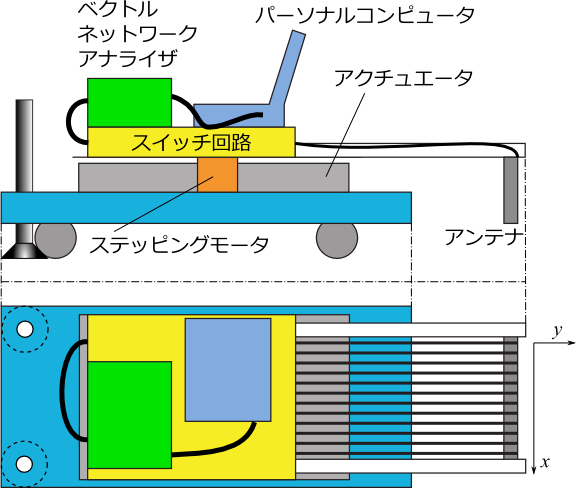
\includegraphics[width =\hsize ]{so2.png}
\caption{1次元アレイアンテナ式地雷可視化システム}
\label{so2}
   \end{minipage}
   \begin{minipage}{0.5\hsize}
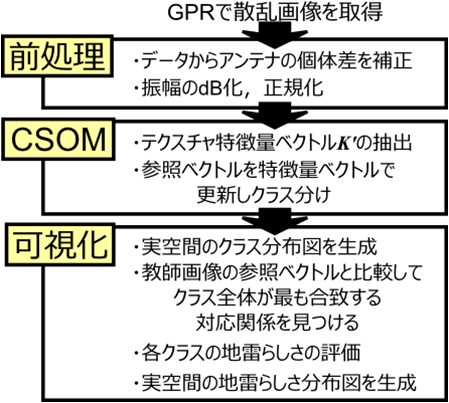
\includegraphics[width =\hsize ]{flowchart.png}
\caption{データ取得から地雷可視化までの流れ}
\label{flow}          
   \end{minipage}
  \end{tabular}
 \end{center}
\end{figure}
\subsection{可視化処理}
\label{021920_15Feb15}
図\ref{flow}にシステムの可視化処理の流れを示す.
事前に補正用のデータを取得しておき,
補正用データを用いて直接結合を減算し,補正後のデータを得る.
その後,振幅をlogスケールにしてdBで表し,正規化
する.ここまでを前処理とし,得られたデータをSOMに掛ける.

まず,$L\times L$ピクセルの局所ウィンドウを設定して,
テクスチャ特徴量を抽出する.
位置$(x,y)$における${\bm K}(x,y)$は,空間的なテクスチャ特徴量
${\it K_{{\rm m}}},{\bm K_{{\rm s}}}$と周波数領域のテクスチャ特徴量
${\bm K_{{\rm f}}}$からなる.
空間的なテクスチャ特徴量は,
各$(l_x,l_y)$の複素画素値の平均${\it K_{{\rm m}}}$,$(l_x,l_y)$の自己相関
${\it K_{{\rm s}}}(0,0)$,$(l_x,l_y)$と$(l_x,l_y+1)$,$(l_x+1,l_y)$,
 $(l_x+1,l_y+1)$との相互相関${\it K_{{\rm s}}}(0,1),
 {\it K_{{\rm s}}}(1,0),{\it K_{{\rm s}}}(1,1)$をとる.
\begin{eqnarray}
{\bm K_{{\rm s}}} &=& \left[\begin{array}{cccc}
 {\it K_{{\rm s}}}(0,0) & {\it K_{{\rm s}}}(0,1) &
 {\it K_{{\rm s}}}(1,0) & {\it K_{{\rm s}}}(1,1)
 \end{array} \right]^{\mathrm{T}}
\end{eqnarray}

ただし$T$は転置を表し,$l_x,l_y$は局所ウィンドウの中の座標であ
り,$N$は周波数領域で使用する画像の数である.
 また周波数領域での特徴量として,$f_{\rm int}$
 高い周波数での同じ位置との相互相関${\bm K_{{\rm f}}}$をとる.
これらの特徴量を式(\ref{eq.K})のように1つのベクトルにまとめている
.
その後,$(x,y)$について掃引し,特徴量ベクトル${\bm K}(x,y)$を次のように得る.
\begin{eqnarray}
{\bm K} = \left[\begin{array}{ccc}
      {\it K_{{\rm m}}} & {\bm K_{{\rm s}}} & {\bm K}_{{\rm f}}
           \end{array} \right]^{\mathrm{T}}\label{eq.K}
\end{eqnarray}
これをSOMに代入する.
最終的に生成されたSOMはクラスごとに色分けされた区分画像となっている.
\section{異方性を軽減する自己組織化マップ}
\subsection{異方的重み付け}
今回発生した縦縞ノイズの影響を抑えるために
縦方向の変化に敏感になるようにCSOMの自己組織化ダイナミクスに異方
性をとり入れた.(発表文献\cite{koyama})
まず,全ての$(x,y)$について特徴量ベクトルの分散共分散行列$\Sigma$を算出する.
次に,特徴量ベクトルの要素のうち異方性があると判明しているものを選定する.
今回は,$K_{{\rm s}}(0,1)$,
$K_{{\rm s}}(1,0)$,
$K_{{\rm s}}(1,1)$
の3要素の間に異方性があると考えた.$\Sigma$からこの3要素同士の共分散行列を抽出
し,行列${\Sigma_w}^{-\frac{1}{2}}$を取得する.これを用いて重み
付けを行う.

\begin{equation}
\Sigma_w = \left(\begin{array}{ccc}
	   I_2& &\Large{0} \\
 &\Sigma_3& \\
\Large{0}& &I_9
		\end{array}
\right) 
\end{equation}

勝者クラスを決定する際に従来はユークリッド距離を用いていた.
\begin{equation}
\tilde{c}_E = \argmin_{c} \|{\bm K} - {\bm w_c} \|\label{192027_15Feb15}
\end{equation}
これを重み付けすると,${\Sigma_w}^{-\frac{1}{2}}$はエルミート行列であるの
で以下のように変形できる.
\begin{eqnarray}
\tilde{c}_E&=&\argmin_{c} \|{\Sigma_w}^{-\frac{1}{2}}\left({\bm K} -
						      {\bm w_c}\right)\|\\
 &=&\argmin_{c} \sqrt{\left({\bm K} - {\bm w_c}\right)^{\dagger}
    {\Sigma_w}^{-1}\left({\bm K} - {\bm w_c}\right)}
\end{eqnarray}
この式から分かるように,異方性のある要素においてはユークリッド距離ではな
くマハラノビス距離となっている.
\subsection{複素内積での勝者クラス決定法}
CSOMで各特徴量ベクトルの入力に対して勝者クラスを決定する方法として,
特徴量ベクトルと参照ベクトルの複素内積を
とり最大となるクラス$\tilde{c}_I$を選択する方法\cite{2010Yoshida}を導入
する.
\begin{eqnarray}
\tilde{c}_I = \argmax_{c} \left( \left|
 \frac{{\bm K}^{\dagger}\cdot{\bm w_c}}{ \|{\bm K}\| \| {\bm w_c} \| }
                                   \right| \right)
\end{eqnarray}
従来の地雷可視化システムでは式(\ref{192027_15Feb15})を選択していた.
しかし,本報告で提案するシステムではコヒーレンスにより敏感な本手法が有
効であると予想できる.

次に,本手法で前項で説明した異方的重み付けを行う場合の条件式を以下に表す.
\begin{eqnarray}
\tilde{c}_I &=& \argmax_{c} \left( \left|
\frac{\left({\Sigma_w}^{-\frac{1}{2}}{\bm K}\right)^{\dagger}\cdot
\left({\Sigma_w}^{-\frac{1}{2}}{\bm w_c}\right)
}{ \|{\Sigma_w}^{-\frac{1}{2}}{\bm K}\| \|{\Sigma_w}^{-\frac{1}{2}}{\bm w_c} \| }
                                   \right| \right)
\end{eqnarray}

\section{模擬地雷計測実験}
\subsection{実験方法}
外径40cmの立方体型の植木鉢を用意し,そこに渇い
た土を入れ模擬地雷
を埋設した.土には小石や小枝などの他の散乱源も多数存在している.
\subsection{計測結果}
図\ref{mine-raw},図\ref{direct-raw}は,GPRからベクトルネットワークアナライザを通じて得られた振幅と
位相のデータを補正前の段階で画像として表示したものである.アンテナの
個体差が縦縞となって表れているのが確認できる.図\ref{mine-raw}は模擬地雷を埋設した
地面を計測したもの,図\ref{direct-raw}は
アンテナ下90cmに何も遮るものがない空間を計測したものである.
図\ref{direct-raw}のデータを直接結合の補正として用いて補正
した結果が図\ref{mine6-hosei}である.前処理では縦縞を軽減することはでき
るものの,完全に除去することはできなかった.
\begin{figure}[hbtp]
 \begin{center}
     \begin{minipage}[c]{0.1\hsize}
振幅
  \end{minipage}
     \begin{minipage}[c]{0.79\hsize}
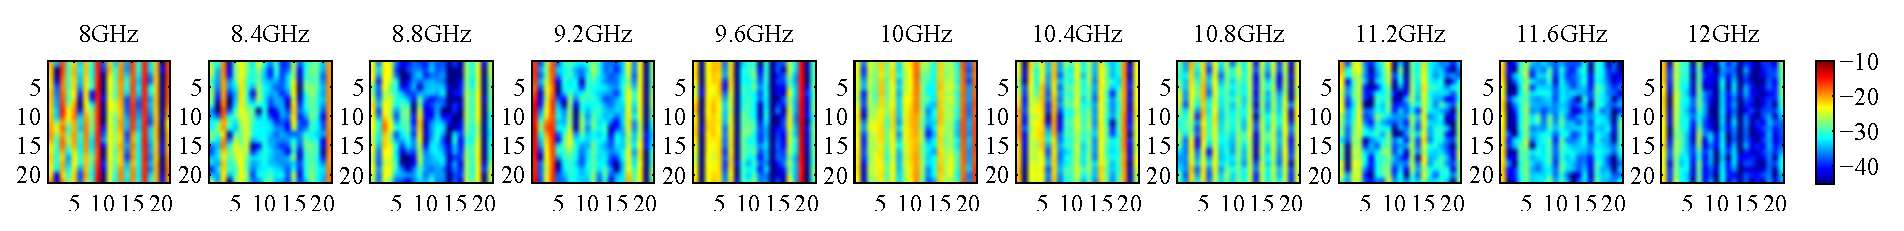
\includegraphics[width = \hsize ]{20150204_mine6_raw_a.eps}
  \end{minipage}
\\
     \begin{minipage}[c]{0.1\hsize}
位相
  \end{minipage}
     \begin{minipage}[c]{0.8\hsize}
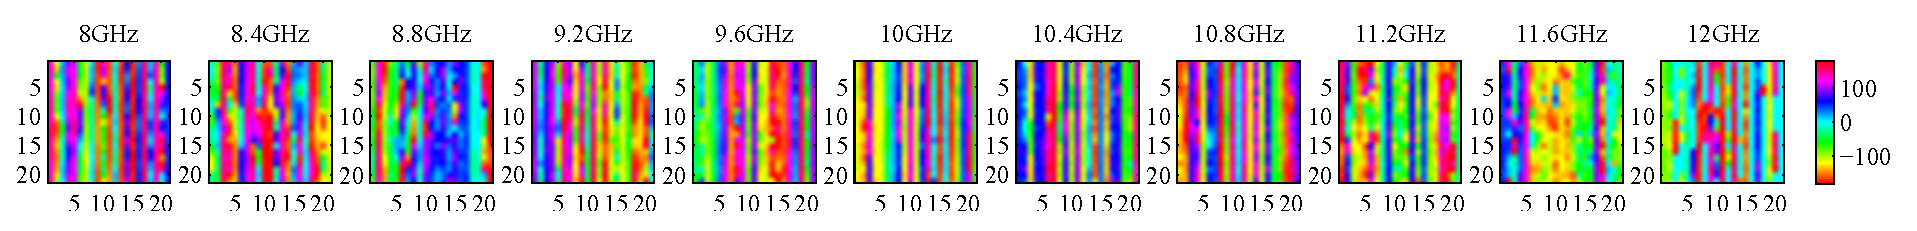
\includegraphics[width =\hsize ]{20150204_mine6_raw_p.eps}
  \end{minipage}
\\
\caption{模擬地雷を埋設して計測したデータ}
\label{mine-raw}
 \end{center}
\end{figure}
\begin{figure}[hbtp]
 \begin{center}
     \begin{minipage}[c]{0.1\hsize}
振幅
  \end{minipage}
     \begin{minipage}[c]{0.79\hsize}
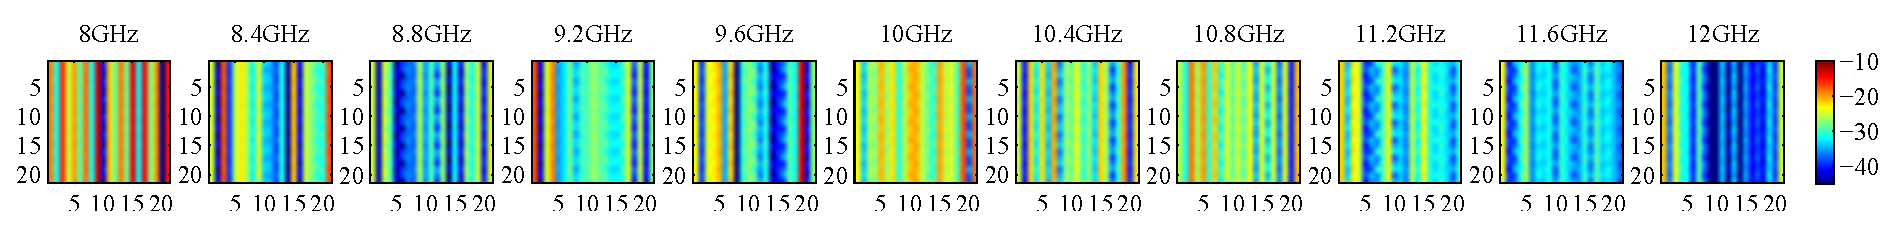
\includegraphics[width = \hsize ]{20150206_direct2_raw_a.eps}
  \end{minipage}
\\
     \begin{minipage}[c]{0.1\hsize}
位相
  \end{minipage}
     \begin{minipage}[c]{0.8\hsize}
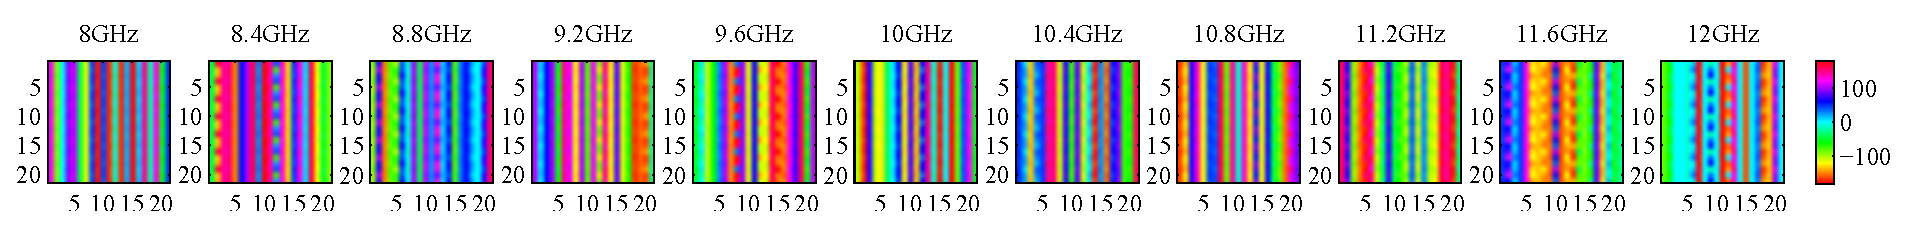
\includegraphics[width =\hsize ]{20150206_direct2_raw_p.eps}
  \end{minipage}
\caption{空中を計測したデータ}
\label{direct-raw}
 \end{center}
\end{figure}
\begin{figure}[hbtp]
 \begin{center}
     \begin{minipage}[c]{0.1\hsize}
振幅
  \end{minipage}
     \begin{minipage}[c]{0.79\hsize}
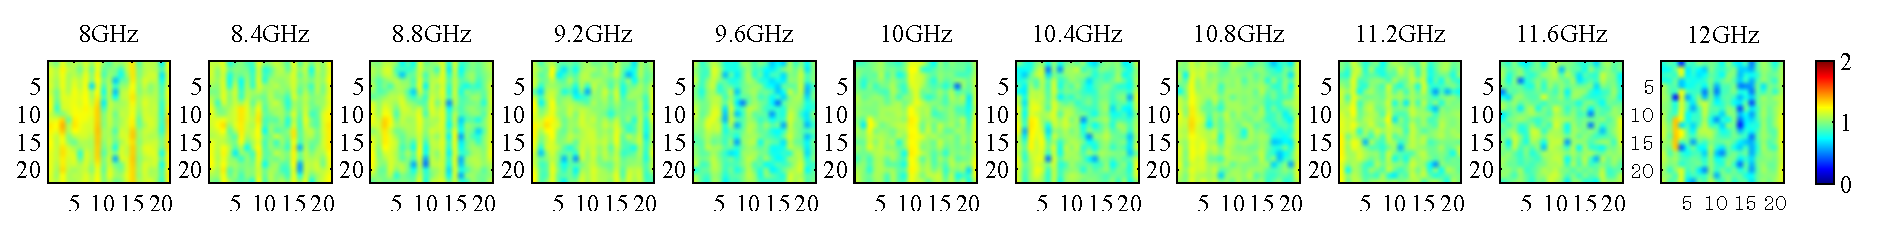
\includegraphics[width = \hsize ]{20150204_mine6_Bhosei_a.eps}
  \end{minipage}
\\
     \begin{minipage}[c]{0.1\hsize}
位相
  \end{minipage}
     \begin{minipage}[c]{0.8\hsize}
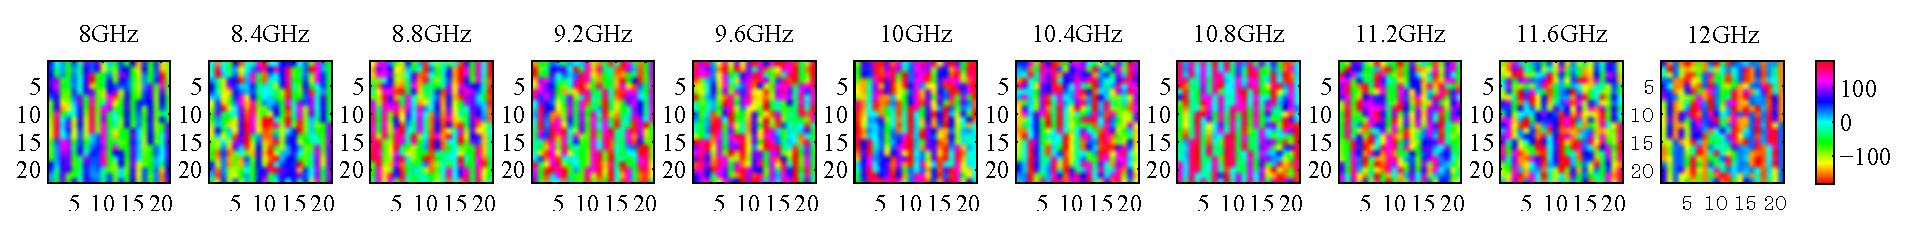
\includegraphics[width =\hsize ]{20150204_mine6_Bhosei_p.eps}
  \end{minipage}
\caption{dataを補正した後の画像}
\label{mine6-hosei}
 \end{center}
\end{figure}

\subsection{2つの新手法と区分画像}
前処理を適用し補正した後の画像に対し,
異方的重み付けと複素内積での勝者クラス決定法を試した.
まず,ユークリッド距離で勝者クラスを決定する従来の手法で異方的重み付け
を行ったSOMの結果が図\ref{aniso-e}である.次に,複素内積を用いた結果が
図\ref{aniso-i}である.

\begin{figure}[btp]
 \begin{center}
   \begin{minipage}{0.4\hsize}
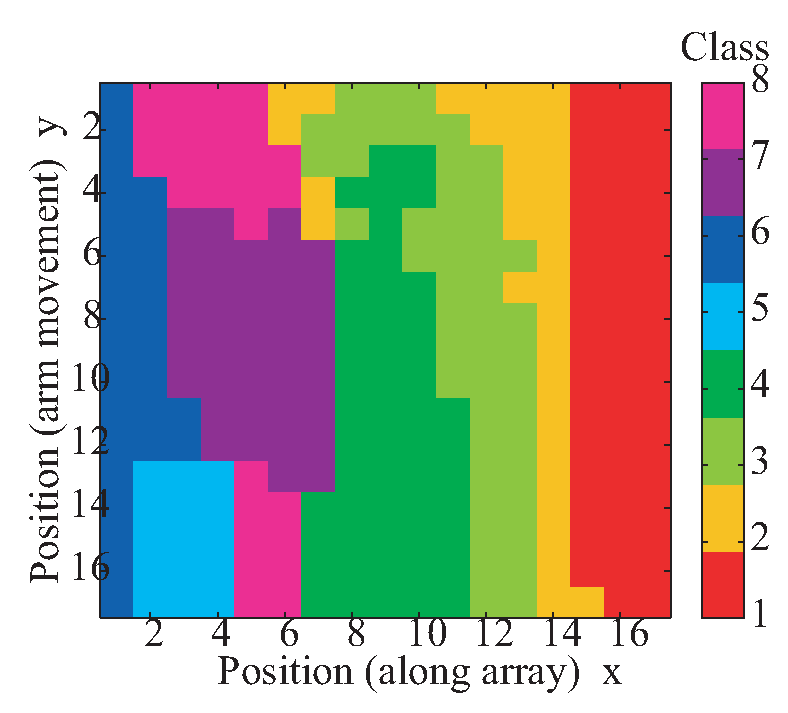
\includegraphics[width =\hsize ]{SOM_mine6_02005_e_raw.eps}
\centering\textmd{異方的重み付けなし}
   \end{minipage}
   \begin{minipage}{0.4\hsize}
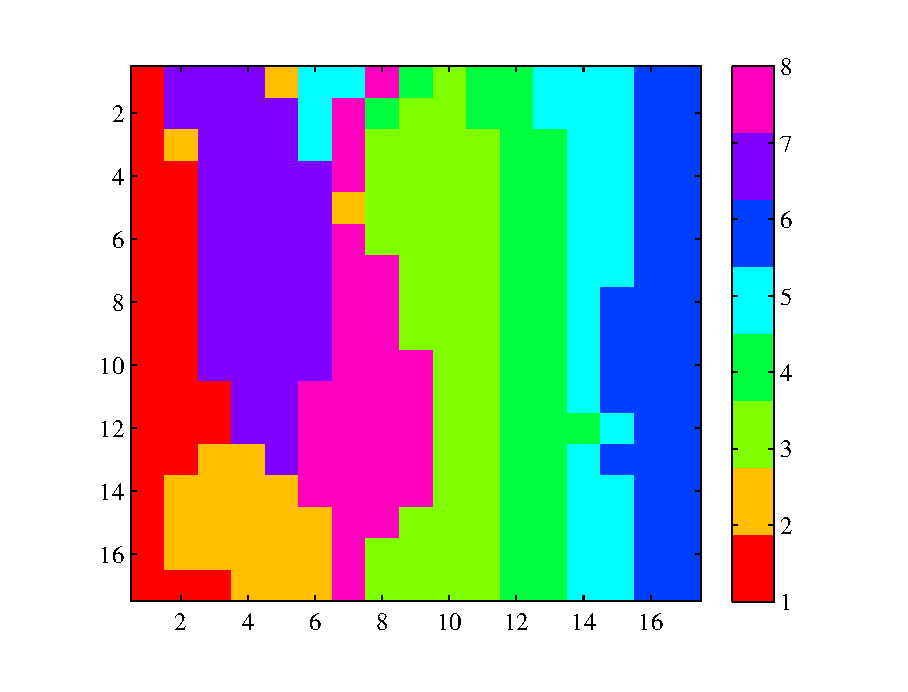
\includegraphics[width =\hsize ]{SOM_mine6_02005_e_wsqrt.eps}
\centering\textmd{異方的重み付けあり}
   \end{minipage}
\caption{ユークリッド距離と異方的重み付け}
\label{aniso-e}
 \end{center}
 \begin{center}
   \begin{minipage}{0.4\hsize}
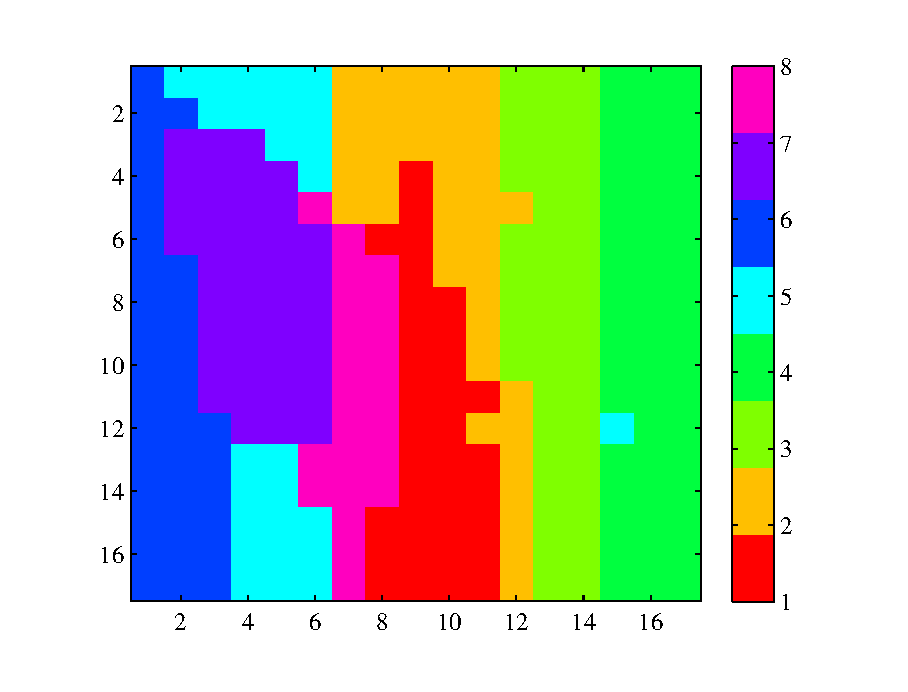
\includegraphics[width =\hsize ]{SOM_mine6_02005_i_raw.eps}
\centering\textmd{異方的重み付けなし}
   \end{minipage}
   \begin{minipage}{0.4\hsize}
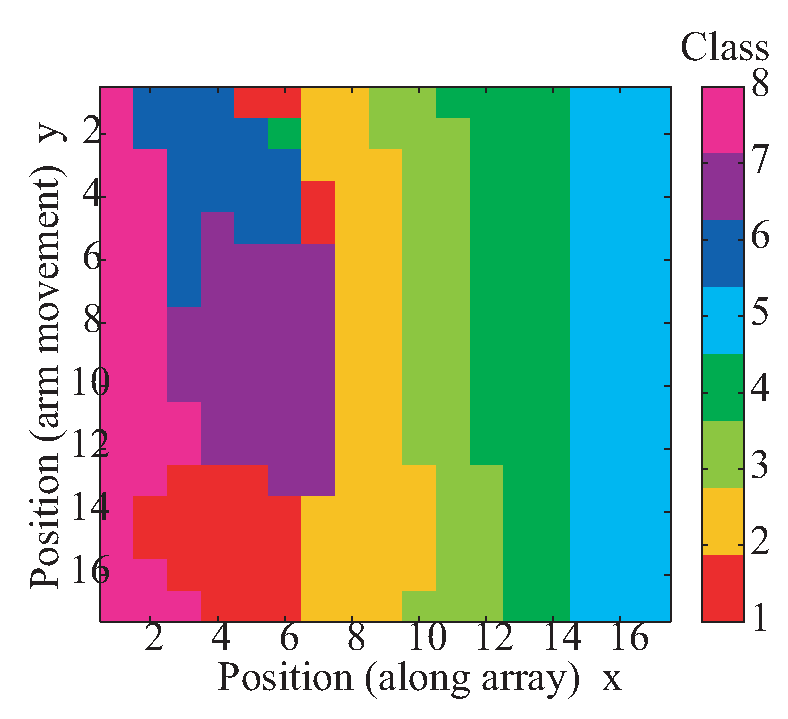
\includegraphics[width =\hsize ]{SOM_mine6_02005_i_wsqrt.eps}
\centering\textmd{異方的重み付けあり}
   \end{minipage}
\caption{複素内積と異方的重み付け}
\label{aniso-i}
 \end{center}
\end{figure}
\section{考察と今後の課題}
\subsection{勝者クラスの決定法の選択}
異方的重み付けを行うことにより,図\ref{aniso-e}において
縦縞の影響が軽減されたことを確認した.しかし,ユークリッド距
離においては異方的重み付けを行うことで地雷クラスの形状が歪んでしまっていた.

複素内積による勝者クラス決定法は,異方的重み付けを行わない場合には,
ユークリッド距離による勝者クラス決定法よりも形状が歪んでいるが,異方
的重み付けを行った際には最も地雷の形状を適切に判断できている.
以上より,4手法の比較において,異方的重み付けを行いつつ複素内積による勝
者クラス決定法を用いるのが適切であると言える.
\subsection{今後の課題}
継続して計測速度を改善しつつ,アンテナ部の機構を見直し性能を向上させる.
また,データ数を増やして実際に未知画像を取得し地雷の判別率を算出,実用性を検討する.
%\bibliography{myrefs}
{\tiny
\begin{thebibliography}{99}% 文献数が10未満の時 {9}
\bibitem{JeroenYarovoy} Jeroen Groenenboom, Alexander Yarovoy,
"Data Processing and Imaging in GPR System Dedicated for Landmine
Detection," Subsurface Sensing Technologies and Applications, vol.3,
        no.4, pp. 387-402, 2002.
 \bibitem{2009Sato} M. Sato, K. Takahashi, "Development of
        Dual Sensors and Deployment in Mine Affected
        Countries," in {\it Anti-personal Landmine Detection for
        Humanitarian Demining}, pp. 27-44, 2009.
\bibitem{2009Nakano} Y. Nakano and A. Hirose, "Improvement of plastic
        landmine visualization performance by use of ring-csom and
        frequency-domain local correlation," IEICE Transactions on
        Electronics, vol. E92-C, no. 1, pp. 102-108, January 2009.
\bibitem{2010Yoshida} A. Hirose and S. Yoshida, "Generalization
        Characteristics of Complex-Valued Feedforward Neural Networks in
        Relation to Signal Coherence," IEEE Neural Networks and Learning
        Systems, vol.23, no.4, 541-551, April 2012.
\end{thebibliography}
\renewcommand{\refname}{発表文献}
\begin{thebibliography}{9}
\bibitem{koyama} E. Koyama, K. Matsuyama, A. Ejiri, and
        A. Hirose, "Landmine visualization system using complex-valued
        self-organizing map with one-dimensional array antenna," IEICE
        Neurocomputing, Technical Report, vol.113, no.500, 
        pp. 69-74, March 2014.
\end{thebibliography}
}
\end{document}
